% !TEX program = pdflatex
\documentclass[13pt,a4paper,oneside]{extreport}

% ============================================================
%  Bao cao Project 1: Tiny shell - myShell
%  Bien dich: pdflatex main.tex
% ============================================================

% Bien dich bang pdfLaTeX tren Overleaf
\usepackage[utf8]{inputenc}
\usepackage[T5]{fontenc}
\usepackage[vietnamese]{babel}
\usepackage{lmodern}

\usepackage[a4paper,top=2.5cm,bottom=2.5cm,left=3.0cm,right=2.2cm]{geometry}
\usepackage{setspace}
\onehalfspacing
\usepackage{graphicx}
\usepackage{float}
\usepackage{caption}
\usepackage{subcaption}
\usepackage{array}
\usepackage{tabularx}
\usepackage{longtable}
\usepackage{booktabs}
\usepackage{multirow}
\usepackage{enumitem}
\usepackage{xcolor}
\usepackage{listings}
\usepackage[most]{tcolorbox}
\usepackage{fancyhdr}
\usepackage{titlesec}
\usepackage{hyperref}
\usepackage{indentfirst}
\usepackage{amsmath}

\hypersetup{
    colorlinks=true,
    linkcolor=black,
    citecolor=black,
    urlcolor=blue,
    pdfauthor={Nhom sinh vien},
    pdftitle={Bao cao Project 1 - Tiny shell}
}

% -------------------- Mau sac --------------------
\definecolor{codebg}{RGB}{248,248,248}
\definecolor{codeframe}{RGB}{210,210,210}
\definecolor{keyword}{RGB}{0,70,140}
\definecolor{comment}{RGB}{80,120,80}
\definecolor{string}{RGB}{150,60,60}
\definecolor{titleblue}{RGB}{35,55,130}

% -------------------- Header/footer --------------------
\pagestyle{fancy}
\fancyhf{}
\lhead{Project 1: Tiny shell}
\rhead{myShell}
\cfoot{\thepage}
\renewcommand{\headrulewidth}{0.4pt}

% -------------------- Dinh dang chapter/section --------------------
\titleformat{\chapter}[display]
  {\normalfont\bfseries\Huge\color{titleblue}}
  {\chaptertitlename\ \thechapter}
  {0.5em}
  {\Huge}
\titlespacing*{\chapter}{0pt}{-10pt}{25pt}

\titleformat{\section}
  {\normalfont\Large\bfseries\color{titleblue}}
  {\thesection}{0.8em}{}
\titleformat{\subsection}
  {\normalfont\large\bfseries}
  {\thesubsection}{0.8em}{}

% -------------------- Listing style --------------------
\lstdefinestyle{mystyle}{
    backgroundcolor=\color{codebg},
    frame=single,
    rulecolor=\color{codeframe},
    basicstyle=\ttfamily\small,
    keywordstyle=\color{keyword}\bfseries,
    commentstyle=\color{comment}\itshape,
    stringstyle=\color{string},
    numbers=left,
    numberstyle=\tiny\color{gray},
    stepnumber=1,
    numbersep=8pt,
    showstringspaces=false,
    breaklines=true,
    breakatwhitespace=true,
    tabsize=4,
    columns=fullflexible,
    keepspaces=true,
    captionpos=b
}
\lstset{style=mystyle}

% -------------------- Box style --------------------
\newtcolorbox{noteBox}[1]{
    enhanced,
    colback=blue!3,
    colframe=titleblue,
    fonttitle=\bfseries,
    title=#1,
    boxrule=0.7pt,
    arc=2mm,
    left=1mm,right=1mm,top=1mm,bottom=1mm
}

\newtcolorbox{resultBox}[1]{
    enhanced,
    colback=green!3,
    colframe=green!40!black,
    fonttitle=\bfseries,
    title=#1,
    boxrule=0.7pt,
    arc=2mm,
    left=1mm,right=1mm,top=1mm,bottom=1mm
}

% -------------------- Thong tin de trong --------------------
\newcommand{\TenTruong}{\dotfill}
\newcommand{\TenKhoa}{\dotfill}
\newcommand{\TenMonHoc}{Hệ điều hành}
\newcommand{\TenGiangVien}{\dotfill}
\newcommand{\TenNhom}{\dotfill}
\newcommand{\TenLop}{\dotfill}
\newcommand{\HocKy}{\dotfill}

\begin{document}

% ============================================================
%  Trang bia
% ============================================================
\begin{titlepage}
\begin{center}
    {\Large \textbf{\TenTruong}}\\[0.3cm]
    {\large \textbf{\TenKhoa}}\\[1.5cm]

    {\Large \textbf{BÁO CÁO PROJECT}}\\[0.4cm]
    {\Large \textbf{MÔN HỌC: \TenMonHoc}}\\[1.2cm]

    \rule{0.85\textwidth}{0.8pt}\\[0.5cm]
    {\Huge \textbf{PROJECT 1: TINY SHELL}}\\[0.25cm]
    {\Large \textbf{Thiết kế và cài đặt shell đơn giản trên Windows}}\\[0.5cm]
    \rule{0.85\textwidth}{0.8pt}\\[1.5cm]
\end{center}

\begin{table}[H]
\centering
\renewcommand{\arraystretch}{1.4}
\begin{tabular}{>{\bfseries}p{5cm}p{8cm}}
Giảng viên hướng dẫn: & \TenGiangVien \\
Nhóm thực hiện:       & \TenNhom \\
Lớp:                  & \TenLop \\
Học kỳ:               & \HocKy \\
\end{tabular}
\end{table}

\vfill
\begin{center}
    {\large Hà Nội, tháng \dotfill\ năm \dotfill}
\end{center}
\end{titlepage}

% ============================================================
%  Bang phan cong
% ============================================================
\chapter*{Bảng phân công công việc}
\addcontentsline{toc}{chapter}{Bảng phân công công việc}

\begin{longtable}{|>{\centering\arraybackslash}p{0.7cm}|p{3.2cm}|p{6.2cm}|>{\centering\arraybackslash}p{2.0cm}|>{\centering\arraybackslash}p{2.0cm}|}
\hline
\textbf{STT} & \textbf{Họ và tên} & \textbf{Công việc chính} & \textbf{Mức độ hoàn thành} & \textbf{Ghi chú} \\
\hline
1 & & Phân tích yêu cầu, thiết kế kiến trúc shell, viết báo cáo & & \\
\hline
2 & & Cài đặt parser, foreground/background process, kiểm thử & & \\
\hline
3 & & Cài đặt built-in commands, quản lý tiến trình, PATH & & \\
\hline
4 & & Chạy thử nghiệm, chụp kết quả, hoàn thiện slide/báo cáo & & \\
\hline
\end{longtable}

\noindent\textbf{Đánh giá chung của nhóm:} \dotfill\\[0.5cm]
\dotfill\\[0.5cm]
\dotfill

\newpage
\tableofcontents
\newpage

% ============================================================
\chapter{Giới thiệu đề tài}

\section{Bối cảnh}

Shell là chương trình trung gian cho phép người dùng nhập lệnh, phân tích lệnh và yêu cầu hệ điều hành thực hiện công việc tương ứng. Trong hệ điều hành, shell không chỉ là giao diện nhập lệnh mà còn là môi trường thực hành nhiều khái niệm cốt lõi như tạo tiến trình, đồng bộ tiến trình cha - con, xử lý tín hiệu bàn phím, quản lý biến môi trường và tổ chức các lệnh nội trú.

Đề tài \textbf{Tiny shell} yêu cầu thiết kế và cài đặt một shell đơn giản trên Windows. Chương trình được đặt tên là \textbf{myShell}, viết bằng ngôn ngữ C theo chuẩn C99 và sử dụng trực tiếp các hàm Win32 API để tạo, theo dõi, dừng, tiếp tục và hủy tiến trình.

\begin{figure}[H]
    \centering
    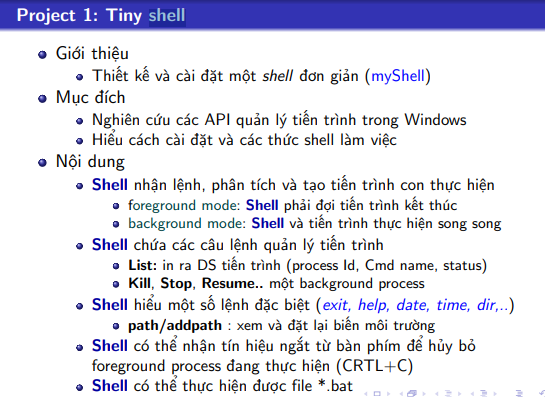
\includegraphics[width=0.88\textwidth]{figures/de_bai.png}
    \caption{Tóm tắt yêu cầu đề bài Project 1: Tiny shell}
\end{figure}

\section{Mục tiêu thực hiện}

Báo cáo tập trung trình bày quá trình thiết kế, cài đặt và kiểm thử shell theo các mục tiêu sau:

\begin{itemize}[leftmargin=1.2cm]
    \item Hiểu cách một shell nhận lệnh, tách tham số và phân loại lệnh.
    \item Cài đặt cơ chế chạy tiến trình ở hai chế độ: \textbf{foreground} và \textbf{background}.
    \item Quản lý danh sách tiến trình chạy nền gồm PID, trạng thái và câu lệnh ban đầu.
    \item Hỗ trợ các thao tác quản lý tiến trình: \texttt{list}, \texttt{kill}, \texttt{stop}, \texttt{resume}.
    \item Cài đặt các lệnh nội trú: \texttt{exit}, \texttt{help}, \texttt{date}, \texttt{time}, \texttt{cd}, \texttt{dir}, \texttt{path}, \texttt{addpath}.
    \item Xử lý tổ hợp phím \texttt{CTRL+C} để hủy foreground process mà không làm chết shell.
    \item Hỗ trợ chạy file batch \texttt{.bat}/\texttt{.cmd} và xây dựng bộ kiểm thử tự động.
\end{itemize}

\section{Phạm vi báo cáo}

Báo cáo này không trình bày toàn bộ mã nguồn dòng theo dòng, mà phân tích các thành phần quan trọng nhất của chương trình: kiến trúc module, cấu trúc dữ liệu, luồng xử lý lệnh, cách gọi Win32 API, kết quả kiểm thử và các hạn chế còn tồn tại. Các đoạn mã trích dẫn trong báo cáo là những phần đại diện cho cơ chế chính của hệ thống.

% ============================================================
\chapter{Cơ sở lý thuyết}

\section{Shell và cơ chế thực thi lệnh}

Một shell dòng lệnh thường hoạt động theo vòng lặp REPL: \textit{Read - Evaluate - Print - Loop}. Ở mỗi vòng lặp, shell in dấu nhắc lệnh, đọc một dòng nhập từ người dùng, phân tích dòng lệnh thành tên lệnh và tham số, sau đó quyết định thực thi lệnh nội trú hoặc tạo tiến trình con để chạy chương trình bên ngoài.

Trong project này, prompt của shell hiển thị theo thư mục hiện tại:

\begin{lstlisting}[language={},caption={Dạng prompt của myShell}]
[C:\Users\admin\OneDrive\Documents\tai lieu\project\shell\shell]>
\end{lstlisting}

Cách hiển thị này giúp người dùng biết shell đang đứng ở thư mục nào và cũng giúp kiểm chứng lệnh \texttt{cd} có làm thay đổi thư mục làm việc của chính shell hay không.

\section{Lệnh nội trú và lệnh ngoài}

Trong shell, cần phân biệt hai loại lệnh:

\begin{table}[H]
\centering
\renewcommand{\arraystretch}{1.25}
\begin{tabularx}{\textwidth}{|p{3.2cm}|X|X|}
\hline
\textbf{Loại lệnh} & \textbf{Đặc điểm} & \textbf{Ví dụ trong project} \\
\hline
Lệnh nội trú & Chạy trực tiếp trong tiến trình shell. Có thể thay đổi trạng thái nội bộ của shell như thư mục hiện tại hoặc biến môi trường. & \texttt{cd}, \texttt{exit}, \texttt{path}, \texttt{addpath}, \texttt{list} \\
\hline
Lệnh ngoài & Shell tạo tiến trình con bằng Win32 API. Tiến trình con có thể chạy foreground hoặc background. & \texttt{notepad}, \texttt{ping}, file \texttt{.bat}/\texttt{.cmd} \\
\hline
\end{tabularx}
\caption{Phân loại lệnh trong myShell}
\end{table}

Lệnh \texttt{cd} là ví dụ điển hình bắt buộc phải là lệnh nội trú. Nếu chạy \texttt{cd} bằng một tiến trình con, thư mục làm việc chỉ thay đổi trong tiến trình con và không ảnh hưởng tới shell cha. Vì vậy chương trình phải gọi \texttt{SetCurrentDirectoryA} ngay trong tiến trình shell.

\section{Foreground process và background process}

Khi chạy lệnh ở chế độ foreground, shell phải chờ tiến trình con kết thúc rồi mới nhận lệnh tiếp theo. Cơ chế này được cài đặt bằng cách gọi \texttt{WaitForSingleObject} trên handle của tiến trình con.

Khi chạy lệnh ở chế độ background, người dùng thêm ký tự \texttt{\&} ở cuối lệnh. Shell tạo tiến trình con nhưng không chờ tiến trình đó kết thúc. Thay vào đó, shell lưu thông tin tiến trình vào danh sách quản lý để người dùng có thể xem, dừng, tiếp tục hoặc hủy tiến trình sau này.

\begin{noteBox}{Ý nghĩa trong hệ điều hành}
Foreground/background là phần thể hiện rõ quan hệ giữa shell và tiến trình con. Foreground yêu cầu đồng bộ tiến trình cha - con, còn background yêu cầu shell duy trì bảng tiến trình riêng để theo dõi những tiến trình chưa kết thúc.
\end{noteBox}

\section{Một số Win32 API được sử dụng}

Project sử dụng trực tiếp các API của Windows thay vì dùng hàm mức cao. Bảng sau tóm tắt những API quan trọng nhất:

\begin{longtable}{|p{4.2cm}|p{10.3cm}|}
\hline
\textbf{API} & \textbf{Vai trò trong chương trình} \\
\hline
\texttt{CreateProcessA} & Tạo tiến trình con để chạy lệnh ngoài hoặc file batch. \\
\hline
\texttt{WaitForSingleObject} & Chờ foreground process kết thúc. \\
\hline
\texttt{TerminateProcess} & Hủy background process theo PID. \\
\hline
\texttt{GetExitCodeProcess} & Kiểm tra tiến trình nền đã kết thúc hay chưa. \\
\hline
\texttt{CloseHandle} & Đóng handle sau khi không còn sử dụng, tránh rò rỉ tài nguyên. \\
\hline
\texttt{SetConsoleCtrlHandler} & Đăng ký hàm xử lý \texttt{CTRL+C}/\texttt{CTRL+BREAK}. \\
\hline
\texttt{GenerateConsoleCtrlEvent} & Gửi \texttt{CTRL\_BREAK\_EVENT} tới nhóm tiến trình foreground. \\
\hline
\texttt{CreateToolhelp32Snapshot} & Chụp danh sách thread trong hệ thống để phục vụ \texttt{stop}/\texttt{resume}. \\
\hline
\texttt{SuspendThread}, \texttt{ResumeThread} & Tạm dừng hoặc tiếp tục từng thread của một background process. \\
\hline
\texttt{SetCurrentDirectoryA} & Thay đổi thư mục làm việc của shell. \\
\hline
\texttt{SetEnvironmentVariableA} & Cập nhật biến môi trường \texttt{PATH} trong phiên shell hiện tại. \\
\hline
\end{longtable}

% ============================================================
\chapter{Phân tích yêu cầu}

\section{Yêu cầu chức năng}

Từ đề bài và kết quả cài đặt, chương trình cần đáp ứng các nhóm chức năng sau:

\begin{longtable}{|p{1.2cm}|p{5cm}|p{8cm}|}
\hline
\textbf{STT} & \textbf{Nhóm yêu cầu} & \textbf{Mô tả} \\
\hline
1 & Nhận và phân tích lệnh & Đọc lệnh từ bàn phím, tách tên lệnh và tham số, nhận biết ký tự \texttt{\&} ở cuối lệnh để chạy nền. \\
\hline
2 & Thực thi foreground & Tạo tiến trình con và chờ tiến trình kết thúc trước khi in prompt mới. \\
\hline
3 & Thực thi background & Tạo tiến trình con, không chờ, lưu PID/trạng thái/câu lệnh vào danh sách quản lý. \\
\hline
4 & Quản lý tiến trình nền & Hỗ trợ \texttt{list}, \texttt{kill <pid>}, \texttt{stop <pid>}, \texttt{resume <pid>}. \\
\hline
5 & Lệnh nội trú cơ bản & Hỗ trợ \texttt{exit}, \texttt{help}, \texttt{date}, \texttt{time}, \texttt{cd}, \texttt{dir}. \\
\hline
6 & Biến môi trường & Hỗ trợ xem \texttt{PATH} và thêm thư mục vào \texttt{PATH} trong phiên hiện tại. \\
\hline
7 & Xử lý \texttt{CTRL+C} & Khi foreground process đang chạy, \texttt{CTRL+C} chỉ hủy tiến trình con, shell vẫn tiếp tục sống. \\
\hline
8 & Batch file & Cho phép chạy file \texttt{.bat}/\texttt{.cmd} bằng cách chuyển qua \texttt{cmd /c}. \\
\hline
9 & Báo lỗi & Khi lệnh sai hoặc API thất bại, in thông báo lỗi dễ hiểu thay vì chỉ in mã lỗi. \\
\hline
\end{longtable}

\section{Yêu cầu phi chức năng}

\begin{itemize}[leftmargin=1.2cm]
    \item Mã nguồn được chia module rõ ràng, mỗi file phụ trách một nhóm chức năng.
    \item Chương trình biên dịch được trên Windows bằng MinGW-w64/GCC.
    \item Có bộ test dạng \texttt{test.bat} để kiểm tra nhanh các chức năng chính.
    \item Khi thoát shell, các background process còn sống được dọn dẹp.
    \item Handle của tiến trình phải được đóng đúng lúc để hạn chế rò rỉ tài nguyên.
\end{itemize}

% ============================================================
\chapter{Thiết kế hệ thống}

\section{Cấu trúc thư mục}

Mã nguồn của project được tổ chức như sau:

\begin{lstlisting}[language={},caption={Cấu trúc thư mục project}]
shell/
|-- Makefile
|-- README.md
|-- test.bat
|-- myShell.exe
`-- src/
    |-- shell.h
    |-- globals.c
    |-- main.c
    |-- parser.h / parser.c
    |-- process.h / process.c
    |-- process_list.h / process_list.c
    |-- builtins.h / builtins.c
    `-- shell_utils.h / shell_utils.c
\end{lstlisting}

\section{Vai trò từng module}

\begin{longtable}{|p{4cm}|p{10.5cm}|}
\hline
\textbf{Module} & \textbf{Vai trò} \\
\hline
\texttt{shell.h} & Khai báo hằng số, kiểu dữ liệu dùng chung, biến toàn cục dùng để theo dõi foreground/background process. \\
\hline
\texttt{globals.c} & Định nghĩa duy nhất các biến toàn cục như \texttt{bg\_procs}, \texttt{bg\_count}, \texttt{g\_fg\_pid}. \\
\hline
\texttt{main.c} & Chứa vòng lặp REPL, in prompt, đăng ký handler \texttt{CTRL+C}, gọi parser và điều phối thực thi lệnh. \\
\hline
\texttt{parser.c} & Tách dòng lệnh thành \texttt{argv}, xử lý dấu nháy, phát hiện trailing \texttt{\&}. \\
\hline
\texttt{process.c} & Xây dựng command line Windows, gọi \texttt{CreateProcessA}, xử lý foreground/background và file batch. \\
\hline
\texttt{process\_list.c} & Quản lý danh sách background process, gồm \texttt{list}, \texttt{kill}, \texttt{stop}, \texttt{resume}, \texttt{reap}. \\
\hline
\texttt{builtins.c} & Cài đặt các lệnh nội trú của shell và kiểm tra lệnh có phải built-in hay không. \\
\hline
\texttt{shell\_utils.c} & Cung cấp hàm báo lỗi thống nhất dựa trên \texttt{FormatMessageA}. \\
\hline
\end{longtable}

\section{Luồng xử lý tổng quát}

\begin{lstlisting}[language={},caption={Luồng xử lý chính của myShell}]
Khoi dong shell
    -> Dang ky CTRL+C handler
    -> Khoi tao danh sach background process
    -> In banner
    -> Lap vo han:
        1. Reap cac background process da ket thuc
        2. In prompt la thu muc hien tai
        3. Doc mot dong lenh
        4. Phan tich lenh thanh argc/argv/background flag
        5. Neu la built-in: chay trong shell process
        6. Neu la lenh ngoai: tao child process bang CreateProcessA
        7. Giai phong bo nho argv
    -> Khi exit: huy cac background process con song
Ket thuc
\end{lstlisting}

\section{Cấu trúc dữ liệu chính}

Hai cấu trúc quan trọng nhất là \texttt{ParsedCmd} và \texttt{BgProcess}. \texttt{ParsedCmd} biểu diễn một lệnh sau khi phân tích. \texttt{BgProcess} biểu diễn một tiến trình nền trong bảng quản lý của shell.

\begin{lstlisting}[language=C,caption={Cấu trúc dữ liệu lệnh và tiến trình nền}]
#define MAX_CMD_LEN     1024
#define MAX_ARGS        64
#define MAX_BG_PROCS    64

typedef enum {
    PROC_RUNNING  = 0,
    PROC_STOPPED  = 1,
    PROC_DONE     = 2
} ProcStatus;

typedef struct {
    DWORD      pid;
    HANDLE     hProcess;
    char       cmd[MAX_CMD_LEN];
    ProcStatus status;
    int        active;
} BgProcess;

typedef struct {
    char  *argv[MAX_ARGS];
    int    argc;
    int    is_background;
} ParsedCmd;
\end{lstlisting}

\section{Thiết kế bảng tiến trình nền}

Chương trình dùng mảng tĩnh \texttt{bg\_procs[MAX\_BG\_PROCS]} với tối đa 64 tiến trình nền. Mỗi phần tử có cờ \texttt{active} để biết slot có đang được dùng hay không. Khi tiến trình kết thúc, hàm \texttt{reap\_processes()} gọi \texttt{GetExitCodeProcess}, đóng handle rồi giải phóng slot.

\begin{noteBox}{Lý do cần reap background process}
Nếu chỉ lưu tiến trình nền nhưng không kiểm tra tiến trình đã kết thúc, danh sách sẽ bị đầy bởi các tiến trình cũ. Ngoài ra, handle của tiến trình đã kết thúc vẫn chiếm tài nguyên hệ thống nếu không gọi \texttt{CloseHandle}.
\end{noteBox}

% ============================================================
\chapter{Cài đặt chi tiết}

\section{Vòng lặp chính trong \texttt{main.c}}

Vòng lặp chính thực hiện đúng mô hình shell: dọn tiến trình nền đã kết thúc, in prompt, đọc dòng lệnh, phân tích, phân loại built-in/external và thực thi.

\begin{lstlisting}[language=C,caption={Rút gọn vòng lặp chính trong main.c}]
while (1) {
    reap_processes();
    print_prompt();

    if (!fgets(line, sizeof(line), stdin)) {
        printf("\n");
        break;
    }

    /* strip newline */
    if (parse_command(line, &cmd) < 0) continue;

    if (is_builtin(&cmd)) {
        int should_exit = run_builtin(&cmd);
        free_parsed_cmd(&cmd);
        if (should_exit) break;
    } else {
        run_process(&cmd);
        free_parsed_cmd(&cmd);
    }
}
\end{lstlisting}

Điểm quan trọng là chương trình gọi \texttt{free\_parsed\_cmd()} sau mỗi lệnh để giải phóng chuỗi \texttt{argv} được cấp phát trong parser.

\section{Phân tích dòng lệnh trong \texttt{parser.c}}

Parser có nhiệm vụ tách dòng nhập thành các tham số giống \texttt{argv}. Phiên bản cài đặt hỗ trợ:

\begin{itemize}[leftmargin=1.2cm]
    \item Bỏ qua khoảng trắng thừa ở đầu/cuối.
    \item Tách token theo khoảng trắng.
    \item Hỗ trợ token có dấu nháy đơn hoặc nháy kép.
    \item Hỗ trợ escape ký tự nháy trong chuỗi được quote.
    \item Phát hiện ký tự \texttt{\&} cuối dòng để đặt \texttt{is\_background = 1}.
    \item Báo lỗi khi thiếu dấu nháy đóng hoặc quá nhiều tham số.
\end{itemize}

\begin{lstlisting}[language=C,caption={Phát hiện background command ở cuối dòng}]
if (!in_quote && end >= 0 && buf[end] == '&') {
    cmd->is_background = 1;
    buf[end] = '\0';
    while (--end >= 0 && (buf[end] == ' ' || buf[end] == '\t')) {
        buf[end] = '\0';
    }
} else if (in_quote) {
    fprintf(stderr, "%s: parse: unmatched quote\n", SHELL_NAME);
    return -1;
}
\end{lstlisting}

Cách làm này bảo đảm dấu \texttt{\&} chỉ có ý nghĩa chạy nền khi nó nằm ở cuối dòng và không nằm trong chuỗi được quote.

\section{Xây dựng command line cho Windows}

Trên Windows, \texttt{CreateProcessA} nhận một chuỗi command line thay vì mảng \texttt{argv} như một số hệ thống Unix. Vì vậy chương trình phải ghép lại các tham số thành một command line hợp lệ. Hàm \texttt{append\_arg()} xử lý trường hợp tham số có khoảng trắng, dấu nháy hoặc dấu gạch chéo ngược.

\begin{lstlisting}[language=C,caption={Rút gọn hàm ghép argv thành command line}]
static int build_cmdline(ParsedCmd *cmd, char *out, int outsize)
{
    int i, pos = 0;
    out[0] = '\0';

    for (i = 0; i < cmd->argc; i++) {
        if (i > 0 && append_char(out, outsize, &pos, ' ') < 0)
            return -1;
        if (append_arg(out, outsize, &pos, cmd->argv[i]) < 0)
            return -1;
    }
    return 0;
}
\end{lstlisting}

Nhờ có bước này, các lệnh chứa đường dẫn có khoảng trắng vẫn có thể được truyền đúng cho tiến trình con.

\section{Tạo foreground/background process}

Hàm \texttt{run\_process()} là phần trung tâm khi chạy lệnh ngoài. Sau khi xây dựng command line, chương trình gọi \texttt{CreateProcessA}. Tất cả tiến trình con được tạo với cờ \texttt{CREATE\_NEW\_PROCESS\_GROUP} để phục vụ xử lý \texttt{CTRL+C} theo nhóm tiến trình.

\begin{lstlisting}[language=C,caption={Gọi CreateProcessA để tạo tiến trình con}]
ok = CreateProcessA(
    NULL,
    final_cmdline,
    NULL,
    NULL,
    TRUE,
    CREATE_NEW_PROCESS_GROUP,
    NULL,
    NULL,
    &si,
    &pi
);

if (!ok) {
    shell_perror(cmd->argv[0]);
    return;
}
\end{lstlisting}

Nếu là foreground process, shell gọi \texttt{WaitForSingleObject} và chỉ quay lại prompt khi tiến trình con kết thúc. Nếu là background process, shell không chờ mà lưu tiến trình vào bảng \texttt{bg\_procs}.

\begin{lstlisting}[language=C,caption={Phân nhánh foreground/background sau khi tạo process}]
if (!cmd->is_background) {
    wait_foreground(&pi);
    CloseHandle(pi.hProcess);
    CloseHandle(pi.hThread);
    return;
}

CloseHandle(pi.hThread);
/* Luu pi.dwProcessId, pi.hProcess, command line vao bg_procs */
\end{lstlisting}

\section{Hỗ trợ file batch}

Windows không chạy trực tiếp file \texttt{.bat}/\texttt{.cmd} như executable thông thường. Vì vậy chương trình kiểm tra phần mở rộng của lệnh. Nếu là file batch, shell tự động thêm tiền tố \texttt{cmd /c}.

\begin{lstlisting}[language=C,caption={Xử lý file .bat/.cmd}]
if (is_batch(cmd->argv[0])) {
    snprintf(final_cmdline, sizeof(final_cmdline), "cmd /c %s", cmdline);
} else {
    strncpy(final_cmdline, cmdline, sizeof(final_cmdline) - 1);
}
\end{lstlisting}

Nhờ đó có thể chạy bộ test bằng cách nhập \texttt{test.bat} trong myShell hoặc dùng lệnh chuyển hướng đầu vào \texttt{.\textbackslash myShell.exe < test.bat}.

\section{Xử lý \texttt{CTRL+C}}

Trong shell thông thường, \texttt{CTRL+C} dùng để hủy chương trình đang chạy foreground. Nếu xử lý không đúng, chính shell cũng bị tắt. Project giải quyết bằng cách đăng ký console control handler bằng \texttt{SetConsoleCtrlHandler}. Khi có foreground process, shell gửi \texttt{CTRL\_BREAK\_EVENT} tới process group của tiến trình đó.

\begin{lstlisting}[language=C,caption={Rút gọn handler xử lý CTRL+C}]
static BOOL WINAPI ctrl_handler(DWORD ctrl_type)
{
    if (ctrl_type == CTRL_C_EVENT || ctrl_type == CTRL_BREAK_EVENT) {
        DWORD pid = g_fg_pid;
        if (pid != 0) {
            GenerateConsoleCtrlEvent(CTRL_BREAK_EVENT, pid);
            return TRUE;
        }
        printf("\n");
        return TRUE;
    }
    return FALSE;
}
\end{lstlisting}

Trong lúc chờ foreground process, biến \texttt{g\_fg\_pid} được gán bằng PID của tiến trình con. Sau khi tiến trình kết thúc, biến này được đặt lại bằng 0.

\section{Quản lý background process}

\subsection{Lệnh \texttt{list}}

Lệnh \texttt{list} in ra bảng gồm PID, trạng thái và command line ban đầu. Trước khi in, chương trình gọi \texttt{reap\_processes()} để loại bỏ các tiến trình đã kết thúc.

\begin{lstlisting}[language=C,caption={In danh sách background process}]
void list_processes(void)
{
    int i, found = 0;
    reap_processes();

    printf("%-8s %-10s %s\n", "PID", "Status", "Command");
    printf("%-8s %-10s %s\n", "---", "------", "-------");

    for (i = 0; i < MAX_BG_PROCS; i++) {
        if (!bg_procs[i].active) continue;
        printf("%-8lu %-10s %s\n",
               (unsigned long)bg_procs[i].pid,
               status_str(bg_procs[i].status),
               bg_procs[i].cmd);
        found++;
    }
    if (!found) printf("(no background processes)\n");
}
\end{lstlisting}

\subsection{Lệnh \texttt{kill}}

Lệnh \texttt{kill <pid>} tìm tiến trình trong bảng nền, gọi \texttt{TerminateProcess}, đóng handle và giải phóng slot.

\begin{lstlisting}[language=C,caption={Hủy background process theo PID}]
int kill_process(DWORD pid)
{
    BgProcess *p = find_proc(pid);
    if (!p) {
        fprintf(stderr, "kill: no background process with PID %lu\n", pid);
        return -1;
    }

    if (!TerminateProcess(p->hProcess, 1)) {
        fprintf(stderr, "kill: TerminateProcess failed\n");
        return -1;
    }

    CloseHandle(p->hProcess);
    p->active = 0;
    p->status = PROC_DONE;
    bg_count--;
    printf("[%lu] Killed\n", pid);
    return 0;
}
\end{lstlisting}

\subsection{Lệnh \texttt{stop} và \texttt{resume}}

Windows không có cơ chế tương đương \texttt{SIGSTOP} đơn giản như trên Unix. Project cài đặt \texttt{stop}/\texttt{resume} bằng cách lấy snapshot danh sách thread trong hệ thống, tìm thread thuộc process cần điều khiển rồi gọi \texttt{SuspendThread} hoặc \texttt{ResumeThread}.

\begin{lstlisting}[language=C,caption={Ý tưởng dừng/tiếp tục toàn bộ thread của một process}]
snap = CreateToolhelp32Snapshot(TH32CS_SNAPTHREAD, 0);
Thread32First(snap, &te);
do {
    if (te.th32OwnerProcessID != pid) continue;
    ht = OpenThread(THREAD_SUSPEND_RESUME, FALSE, te.th32ThreadID);
    if (suspend)
        SuspendThread(ht);
    else
        ResumeThread(ht);
    CloseHandle(ht);
} while (Thread32Next(snap, &te));
\end{lstlisting}

Sau khi thao tác thành công, shell cập nhật trạng thái nội bộ thành \texttt{PROC\_STOPPED} hoặc \texttt{PROC\_RUNNING}.

\section{Cài đặt các lệnh built-in}

Các built-in được khai báo trong mảng \texttt{BUILTIN\_NAMES}. Hàm \texttt{is\_builtin()} so sánh không phân biệt hoa thường bằng \texttt{\_stricmp}. Khi chạy built-in, chương trình không cho phép chạy nền. Nếu người dùng nhập \texttt{date \&}, shell báo lỗi vì built-in phải chạy trong chính shell process.

\begin{lstlisting}[language=C,caption={Danh sách built-in commands}]
static const char *BUILTIN_NAMES[] = {
    "exit", "help", "date", "time", "dir", "cd",
    "list", "kill", "stop", "resume",
    "path", "addpath",
    NULL
};
\end{lstlisting}

Bảng dưới đây tóm tắt các built-in đã cài đặt:

\begin{longtable}{|p{3.2cm}|p{11cm}|}
\hline
\textbf{Lệnh} & \textbf{Cơ chế cài đặt} \\
\hline
\texttt{exit} & Gọi \texttt{kill\_all\_processes()} để dọn tiến trình nền, in \texttt{Goodbye!}, trả về tín hiệu thoát vòng lặp. \\
\hline
\texttt{help} & In bảng hướng dẫn các nhóm lệnh. \\
\hline
\texttt{date}, \texttt{time} & Gọi \texttt{GetLocalTime}, định dạng ngày \texttt{YYYY-MM-DD} và giờ \texttt{HH:MM:SS}. \\
\hline
\texttt{cd [path]} & Không có tham số thì in thư mục hiện tại; có tham số thì gọi \texttt{SetCurrentDirectoryA}. \\
\hline
\texttt{dir [path]} & Tạo process chạy \texttt{cmd /c dir}, cho phép dùng chức năng liệt kê thư mục sẵn có của Windows. \\
\hline
\texttt{path} & Đọc biến môi trường \texttt{PATH} bằng \texttt{getenv}, tách theo dấu chấm phẩy và in từng dòng. \\
\hline
\texttt{addpath <dir>} & Ghép thư mục mới vào cuối \texttt{PATH} và gọi \texttt{SetEnvironmentVariableA}. \\
\hline
\texttt{list}, \texttt{kill}, \texttt{stop}, \texttt{resume} & Gọi các hàm tương ứng trong \texttt{process\_list.c}. \\
\hline
\end{longtable}

\section{Báo lỗi thống nhất}

Thay vì in mã lỗi thô từ \texttt{GetLastError}, project xây dựng hàm \texttt{shell\_perror()} dùng \texttt{FormatMessageA} để chuyển mã lỗi Windows thành chuỗi dễ hiểu.

\begin{lstlisting}[language=C,caption={Hàm báo lỗi dùng FormatMessageA}]
void shell_perror(const char *context)
{
    DWORD err = GetLastError();
    char msg[512];

    FormatMessageA(FORMAT_MESSAGE_FROM_SYSTEM |
                   FORMAT_MESSAGE_IGNORE_INSERTS,
                   NULL, err,
                   MAKELANGID(LANG_NEUTRAL, SUBLANG_DEFAULT),
                   msg, sizeof(msg) - 1, NULL);

    fprintf(stderr, "%s: %s: %s (error %lu)\n",
            SHELL_NAME, context, msg, (unsigned long)err);
}
\end{lstlisting}

Nhờ đó, khi người dùng nhập lệnh sai hoặc đường dẫn không tồn tại, shell in được thông báo có ngữ cảnh như \texttt{myShell: cd: The system cannot find the path specified.}

% ============================================================
\chapter{Biên dịch và kiểm thử}

\section{Môi trường biên dịch}

Project được biên dịch trên Windows bằng GCC/MinGW-w64. Có hai cách biên dịch:

\begin{lstlisting}[language={},caption={Biên dịch trực tiếp bằng gcc}]
gcc -Wall -O2 -std=c99 -D_WIN32_WINNT=0x0600 -Isrc -o myShell.exe ^
    src/main.c src/globals.c src/parser.c src/process.c ^
    src/process_list.c src/builtins.c src/shell_utils.c -lkernel32
\end{lstlisting}

Hoặc dùng Makefile:

\begin{lstlisting}[language={},caption={Biên dịch bằng Makefile}]
mingw32-make
\end{lstlisting}

Trong Makefile, các file nguồn được biên dịch thành object rồi liên kết thành \texttt{myShell.exe}. Các thư viện liên kết gồm \texttt{kernel32} và \texttt{user32} để dùng Win32 API.

\section{Kịch bản kiểm thử}

Bộ kiểm thử \texttt{test.bat} được dùng để kiểm tra tự động những chức năng cơ bản. Ngoài ra, một số chức năng tương tác như \texttt{notepad \&}, \texttt{stop}, \texttt{resume}, \texttt{kill} và \texttt{CTRL+C} được kiểm thử thủ công.

\begin{longtable}{|p{1.2cm}|p{4.2cm}|p{5.4cm}|p{3.5cm}|}
\hline
\textbf{STT} & \textbf{Lệnh kiểm thử} & \textbf{Mục tiêu} & \textbf{Kết quả} \\
\hline
1 & \texttt{help} & In bảng lệnh hỗ trợ & Đạt \\
\hline
2 & \texttt{date}, \texttt{time} & In ngày/giờ hiện tại đúng định dạng & Đạt \\
\hline
3 & \texttt{cd}, \texttt{cd src}, \texttt{cd ..} & Thay đổi và in thư mục hiện tại & Đạt \\
\hline
4 & \texttt{dir} & Liệt kê nội dung thư mục hiện tại & Đạt \\
\hline
5 & \texttt{cd C:\textbackslash this\_path\_does\_not\_exist\_xyz} & Báo lỗi đường dẫn không tồn tại & Đạt \\
\hline
6 & \texttt{path} & In các entry của biến \texttt{PATH} & Đạt \\
\hline
7 & \texttt{addpath C:\textbackslash mytest\_temp\_dir} & Thêm entry mới vào \texttt{PATH} trong phiên shell & Đạt \\
\hline
8 & \texttt{notepad \&} & Chạy tiến trình nền và lưu PID & Đạt \\
\hline
9 & \texttt{list} & Hiển thị danh sách background process & Đạt \\
\hline
10 & \texttt{stop <pid>} & Tạm dừng tiến trình nền & Đạt \\
\hline
11 & \texttt{resume <pid>} & Tiếp tục tiến trình đã dừng & Đạt \\
\hline
12 & \texttt{kill <pid>} & Hủy tiến trình nền & Đạt \\
\hline
13 & \texttt{kill abc}, \texttt{stop abc}, \texttt{resume abc} & Kiểm tra báo lỗi PID không hợp lệ & Đạt \\
\hline
14 & \texttt{date \&}, \texttt{help \&}, \texttt{dir \&} & Không cho built-in chạy background & Đạt \\
\hline
15 & \texttt{test.bat} & Chạy bộ test batch & Đạt \\
\hline
\end{longtable}

\section{Kết quả chạy chương trình}

\subsection{Khởi động shell và lệnh \texttt{help}}

Khi chạy \texttt{myShell.exe}, chương trình in banner giới thiệu. Lệnh \texttt{help} hiển thị bảng các built-in commands, nhóm quản lý tiến trình và nhóm biến môi trường.

\begin{figure}[H]
    \centering
    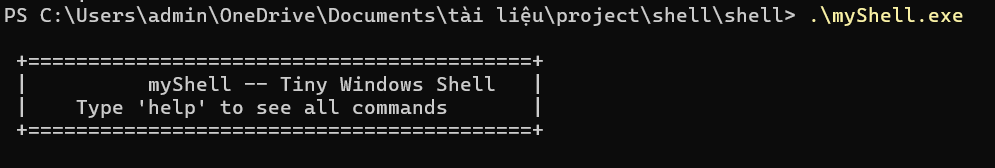
\includegraphics[width=0.82\textwidth]{figures/ketqua_banner.png}
    \caption{Khởi động myShell}
\end{figure}

\begin{figure}[H]
    \centering
    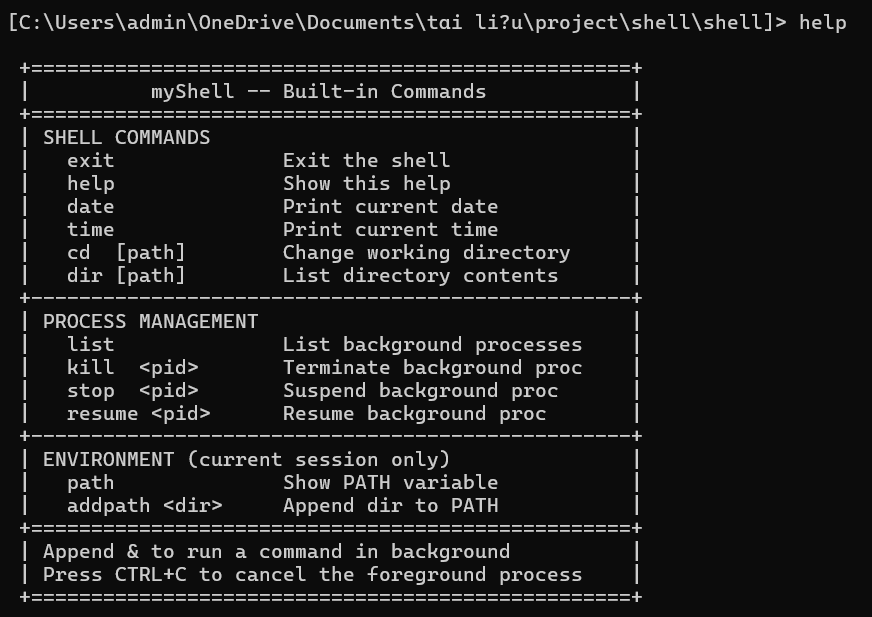
\includegraphics[width=0.82\textwidth]{figures/ketqua_help.png}
    \caption{Kết quả lệnh help}
\end{figure}

\subsection{Kiểm thử ngày, giờ và thư mục hiện tại}

Các lệnh \texttt{date} và \texttt{time} in đúng định dạng. Lệnh \texttt{cd} không tham số in thư mục hiện tại; lệnh \texttt{cd src} và \texttt{cd ..} thay đổi prompt tương ứng.

\begin{figure}[H]
    \centering
    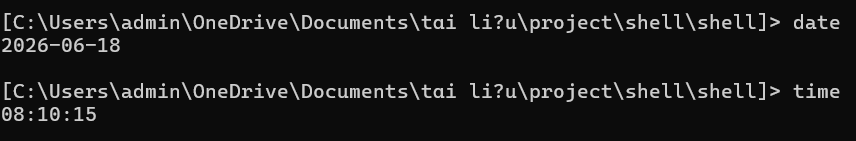
\includegraphics[width=0.82\textwidth]{figures/ketqua_date_time.png}
    \caption{Kết quả lệnh date và time}
\end{figure}

\begin{figure}[H]
    \centering
    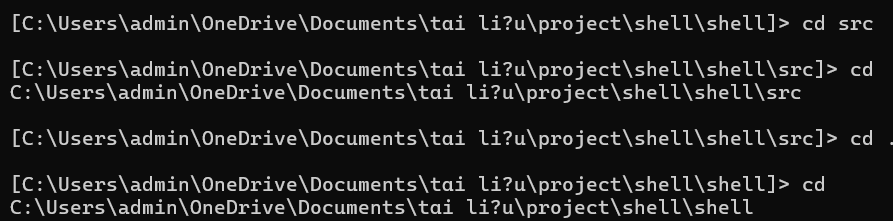
\includegraphics[width=0.82\textwidth]{figures/ketqua_cd.png}
    \caption{Kết quả kiểm thử lệnh cd}
\end{figure}

\subsection{Kiểm thử \texttt{dir}, lỗi đường dẫn và biến môi trường}

Lệnh \texttt{dir} liệt kê nội dung thư mục. Khi nhập đường dẫn sai, shell báo lỗi có nội dung lấy từ hệ thống Windows. Lệnh \texttt{path} in biến môi trường theo từng dòng, còn \texttt{addpath} thêm thư mục mới vào cuối \texttt{PATH} trong phiên hiện tại.

\begin{figure}[H]
    \centering
    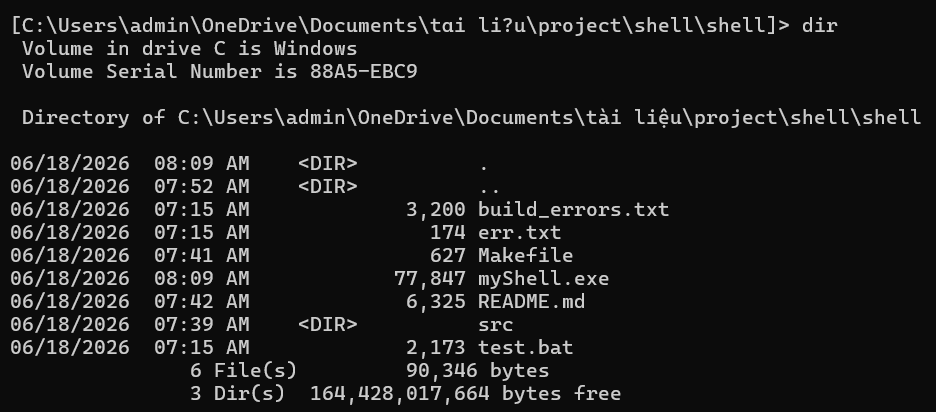
\includegraphics[width=0.88\textwidth]{figures/ketqua_dir.png}
    \caption{Kết quả lệnh dir}
\end{figure}

\begin{figure}[H]
    \centering
    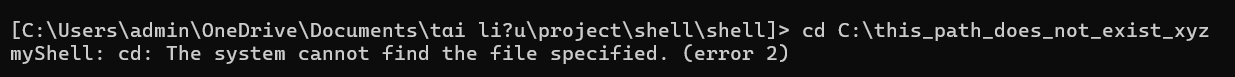
\includegraphics[width=0.82\textwidth]{figures/ketqua_cd_error.png}
    \caption{Kết quả báo lỗi khi cd tới đường dẫn không tồn tại}
\end{figure}

\begin{figure}[H]
    \centering
    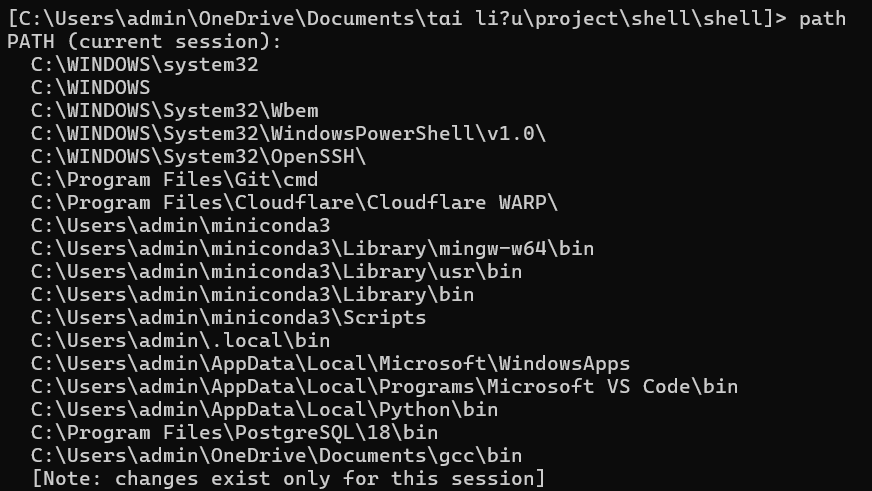
\includegraphics[width=0.82\textwidth]{figures/ketqua_path.png}
    \caption{Kết quả lệnh path}
\end{figure}

\begin{figure}[H]
    \centering
    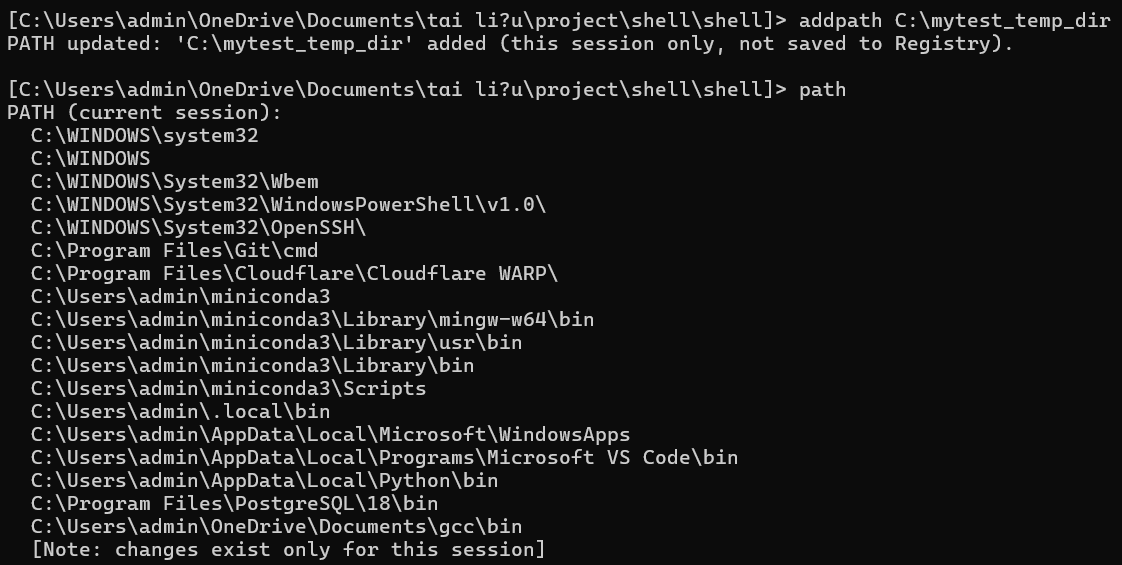
\includegraphics[width=0.82\textwidth]{figures/ketqua_addpath.png}
    \caption{Kết quả lệnh addpath và kiểm tra lại PATH}
\end{figure}

\subsection{Kiểm thử background process}

Lệnh \texttt{notepad \&} tạo tiến trình nền, in PID và cho shell tiếp tục nhận lệnh. Sau đó \texttt{list} hiển thị trạng thái \texttt{Running}. Các lệnh \texttt{stop}, \texttt{resume}, \texttt{kill} cập nhật trạng thái tiến trình đúng như yêu cầu.

\begin{figure}[H]
    \centering
    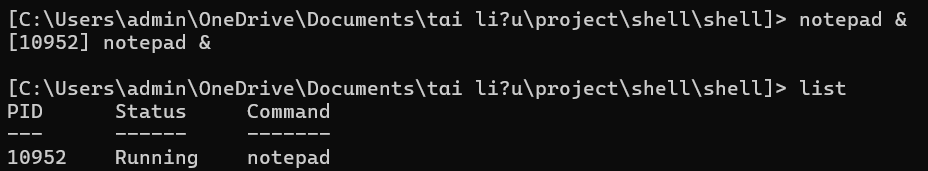
\includegraphics[width=0.82\textwidth]{figures/ketqua_background_start.png}
    \caption{Tạo background process bằng notepad \&}
\end{figure}

\begin{figure}[H]
    \centering
    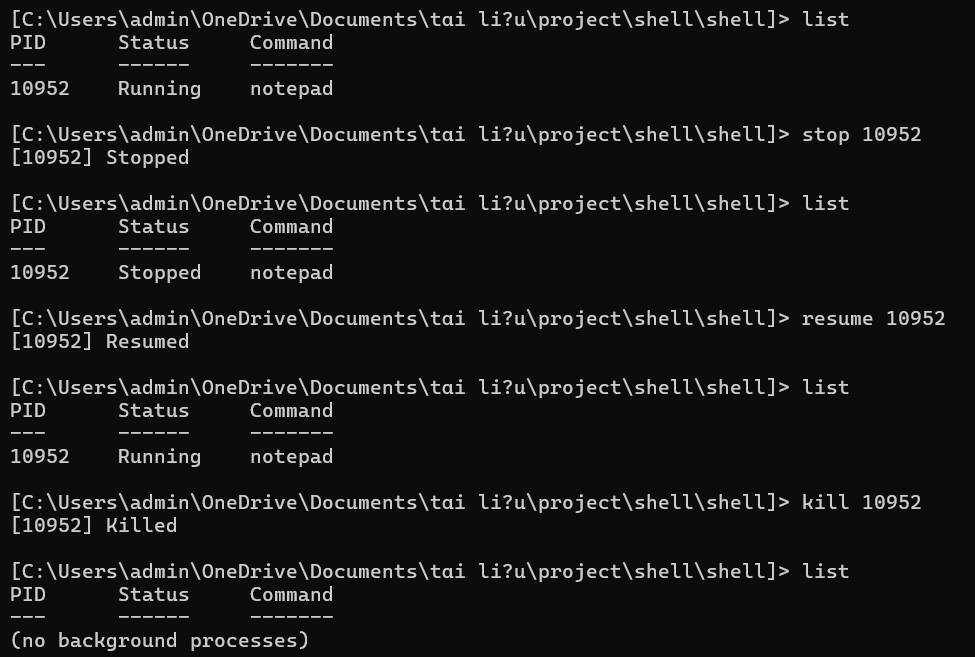
\includegraphics[width=0.82\textwidth]{figures/ketqua_background_manage.png}
    \caption{Kiểm thử list, stop, resume và kill với background process}
\end{figure}

\subsection{Kiểm thử trường hợp lỗi}

Với PID không hợp lệ như \texttt{abc}, các lệnh \texttt{kill}, \texttt{stop}, \texttt{resume} đều báo lỗi rõ ràng. Khi cố chạy built-in ở background, shell từ chối vì built-in phải chạy trong shell process.

\begin{figure}[H]
    \centering
    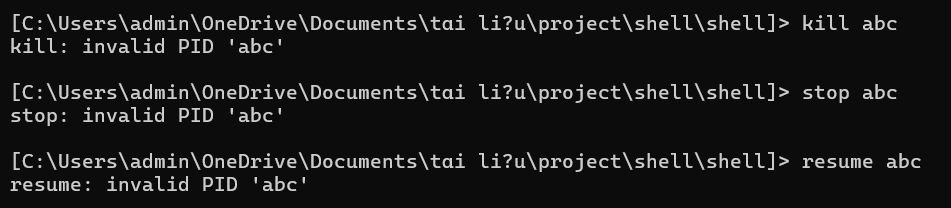
\includegraphics[width=0.82\textwidth]{figures/ketqua_invalid_pid.png}
    \caption{Báo lỗi khi PID không hợp lệ}
\end{figure}

\begin{figure}[H]
    \centering
    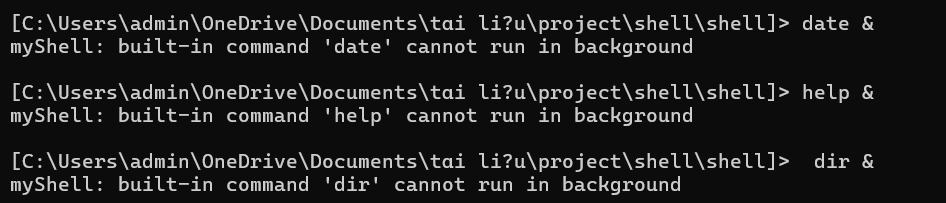
\includegraphics[width=0.82\textwidth]{figures/ketqua_builtin_bg.png}
    \caption{Báo lỗi khi cố chạy built-in command ở background}
\end{figure}

\subsection{Kiểm thử bằng \texttt{test.bat}}

File \texttt{test.bat} chạy lần lượt các test tự động: ngày, giờ, liệt kê thư mục, đổi thư mục, đường dẫn sai, PATH, addpath, list, foreground process bằng \texttt{ping} và help. Cuối file có gợi ý các test thủ công cho background process và \texttt{CTRL+C}.

\begin{figure}[H]
    \centering
    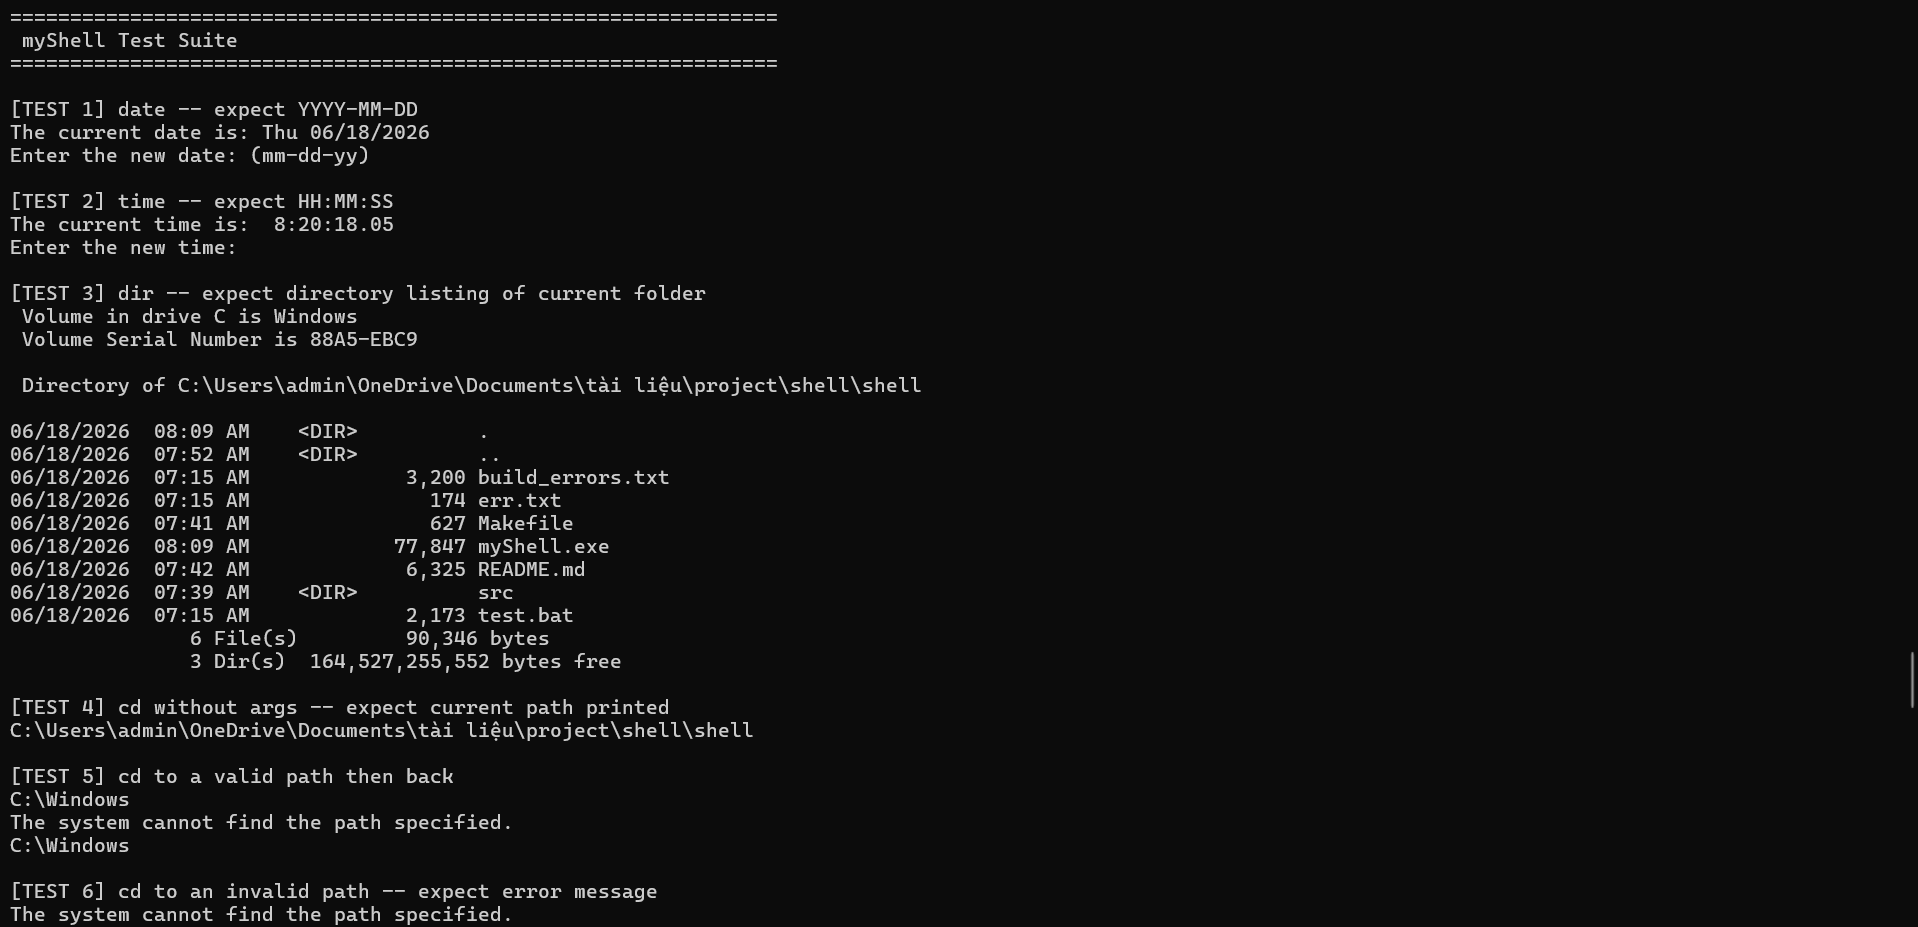
\includegraphics[width=0.88\textwidth]{figures/ketqua_test_1.png}
    \caption{Một phần kết quả chạy test.bat - nhóm test đầu}
\end{figure}

\begin{figure}[H]
    \centering
    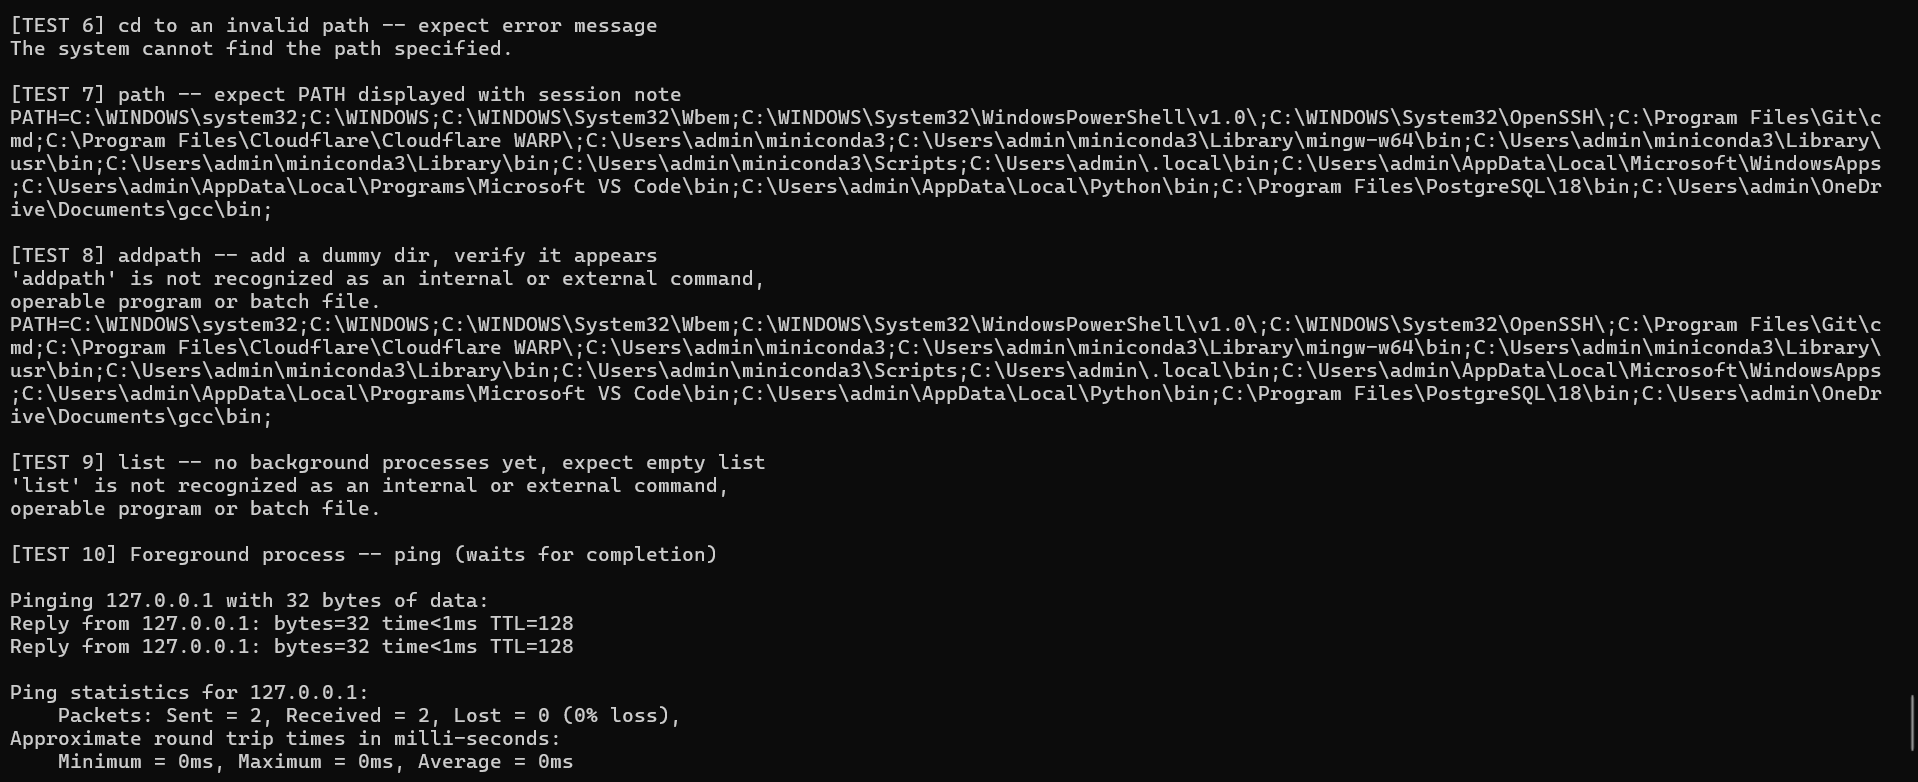
\includegraphics[width=0.88\textwidth]{figures/ketqua_test_2.png}
    \caption{Một phần kết quả chạy test.bat - kiểm tra PATH, addpath, list và ping}
\end{figure}

\begin{figure}[H]
    \centering
    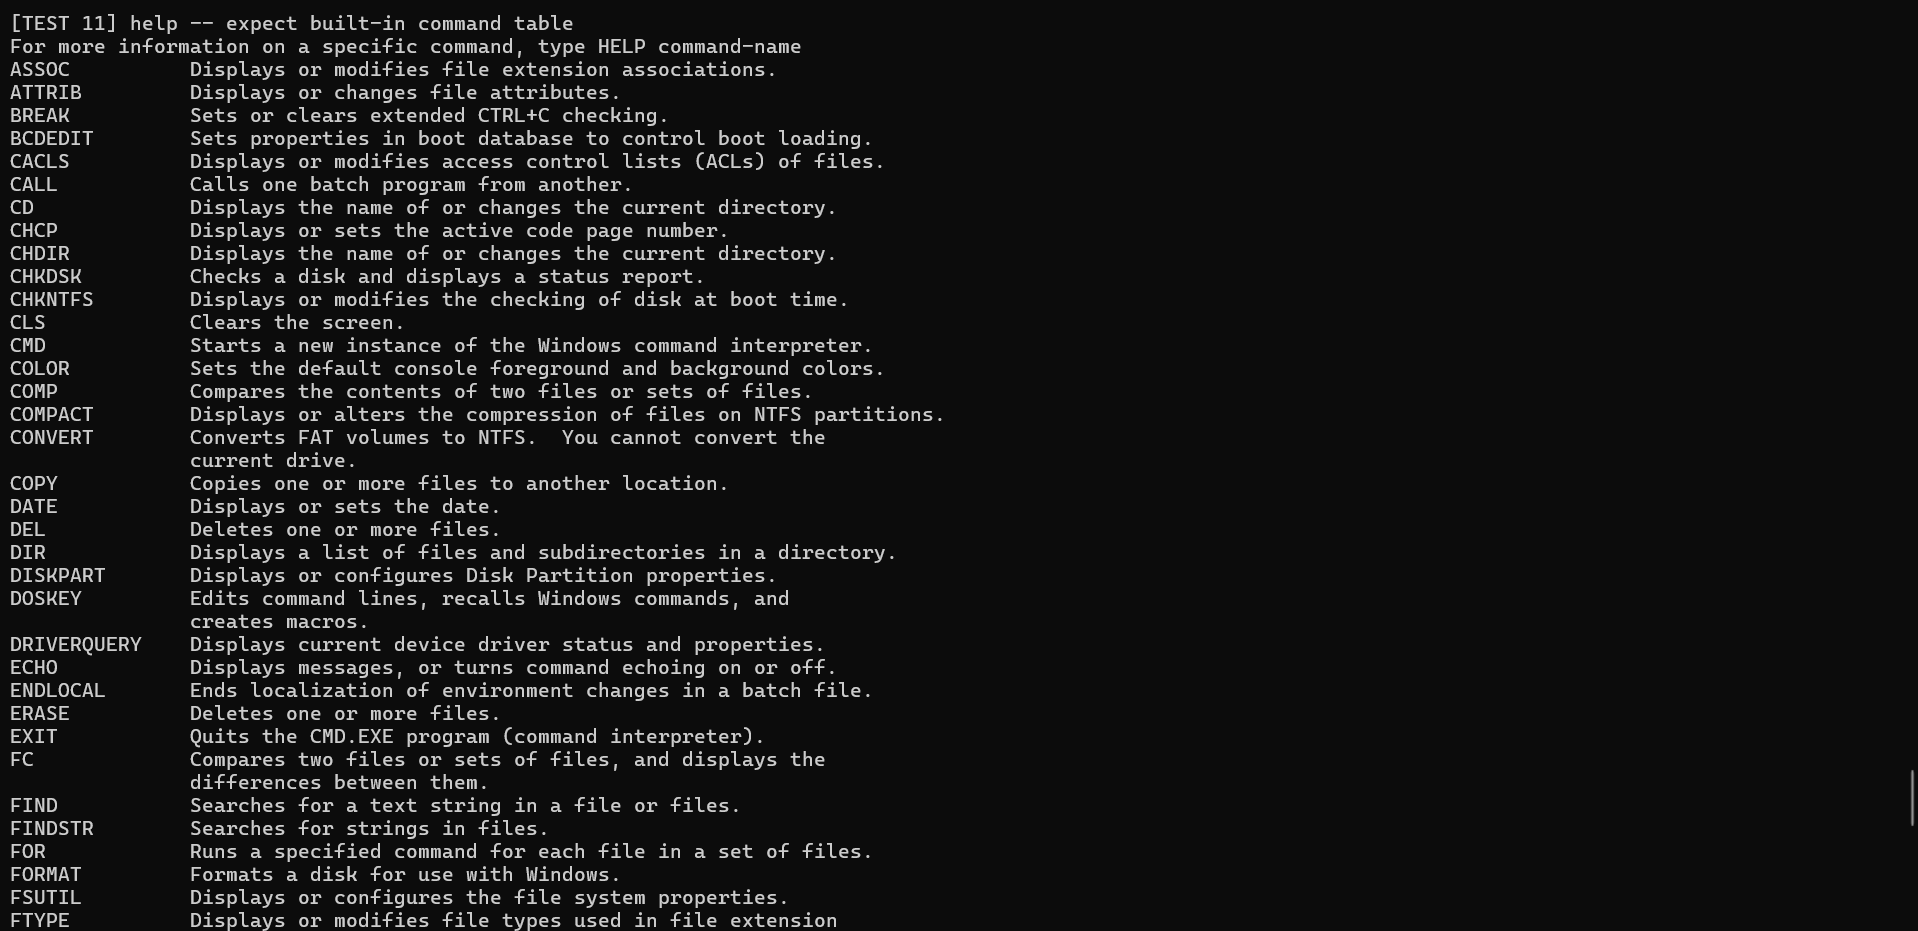
\includegraphics[width=0.88\textwidth]{figures/ketqua_test_3.png}
    \caption{Một phần kết quả chạy test.bat - bảng help}
\end{figure}

\begin{resultBox}{Nhận xét kết quả}
Các kết quả chạy trên máy cá nhân cho thấy shell đáp ứng các yêu cầu chính của đề bài: nhận lệnh, chạy foreground/background process, quản lý background process, xử lý built-in command, cập nhật PATH trong phiên hiện tại, chạy batch file và báo lỗi với các trường hợp nhập sai.
\end{resultBox}

% ============================================================
\chapter{Đánh giá và thảo luận}

\section{Các yêu cầu đã hoàn thành}

\begin{table}[H]
\centering
\renewcommand{\arraystretch}{1.25}
\begin{tabularx}{\textwidth}{|p{1.2cm}|X|p{3cm}|}
\hline
\textbf{STT} & \textbf{Yêu cầu} & \textbf{Trạng thái} \\
\hline
1 & Shell nhận lệnh, phân tích tham số và tạo tiến trình con & Hoàn thành \\
\hline
2 & Foreground mode: shell chờ tiến trình con kết thúc & Hoàn thành \\
\hline
3 & Background mode: shell và tiến trình chạy song song & Hoàn thành \\
\hline
4 & Quản lý tiến trình nền bằng list/kill/stop/resume & Hoàn thành \\
\hline
5 & Built-in commands: exit/help/date/time/cd/dir/path/addpath & Hoàn thành \\
\hline
6 & \texttt{CTRL+C} hủy foreground process, shell tiếp tục sống & Hoàn thành \\
\hline
7 & Hỗ trợ file \texttt{.bat}/\texttt{.cmd} & Hoàn thành \\
\hline
8 & Báo lỗi Win32 rõ ràng bằng \texttt{FormatMessageA} & Hoàn thành \\
\hline
\end{tabularx}
\caption{Tổng hợp mức độ hoàn thành yêu cầu}
\end{table}

\section{Ưu điểm của cài đặt}

\begin{itemize}[leftmargin=1.2cm]
    \item Mã nguồn được chia module theo đúng trách nhiệm, dễ đọc và dễ mở rộng.
    \item Không chỉ tạo tiến trình mà còn quản lý được vòng đời tiến trình nền.
    \item Có cơ chế \texttt{reap\_processes()} để đóng handle và giải phóng slot khi process kết thúc.
    \item Xử lý \texttt{CTRL+C} theo process group, tránh làm chết shell.
    \item Hỗ trợ batch file nên có thể kiểm thử bằng script tự động.
    \item Các lỗi Win32 được in thành thông báo dễ hiểu cho người dùng.
\end{itemize}

\section{Hạn chế}

\subsection{Giới hạn của \texttt{stop}/\texttt{resume}}

Cơ chế \texttt{stop}/\texttt{resume} dựa trên \texttt{SuspendThread}/\texttt{ResumeThread}. Cách này phù hợp với project học thuật nhưng có rủi ro trong môi trường thực tế:

\begin{itemize}[leftmargin=1.2cm]
    \item Nếu thread bị suspend khi đang giữ lock quan trọng, chương trình có thể bị deadlock.
    \item Nếu process tạo thêm thread sau thời điểm snapshot, thread mới có thể không bị suspend.
    \item Windows không có một API đơn giản tương đương \texttt{SIGSTOP} để dừng an toàn toàn bộ process theo kiểu Unix.
\end{itemize}

\subsection{Phạm vi của \texttt{addpath}}

Lệnh \texttt{addpath} chỉ thay đổi biến \texttt{PATH} trong tiến trình shell hiện tại. Thay đổi này được các tiến trình con tạo sau đó kế thừa, nhưng không được ghi vào Registry nên sẽ mất khi thoát shell.

\subsection{Command dispatcher còn có thể tối ưu}

Hiện tại, hàm \texttt{run\_builtin()} dùng chuỗi \texttt{if}/\texttt{strcmp} để gọi từng built-in. Khi số lượng lệnh tăng, nên chuyển sang bảng dispatch gồm tên lệnh và con trỏ hàm để việc mở rộng dễ hơn.

\section{Hướng phát triển}

\begin{itemize}[leftmargin=1.2cm]
    \item Bổ sung chuyển hướng vào/ra file: \texttt{>}, \texttt{>>}, \texttt{<}.
    \item Hỗ trợ pipeline: \texttt{cmd1 | cmd2}.
    \item Thêm lịch sử lệnh và phím mũi tên để gọi lại lệnh cũ.
    \item Cải tiến parser để hỗ trợ nhiều cú pháp đặc biệt hơn của Windows command line.
    \item Dùng bảng dispatch để quản lý built-in command chuyên nghiệp hơn.
    \item Dùng Windows Job Object để quản lý nhóm tiến trình nền an toàn hơn.
\end{itemize}

% ============================================================
\chapter{Kết luận}

Project \textbf{Tiny shell - myShell} đã cài đặt được một shell đơn giản trên Windows với các chức năng chính của đề bài. Chương trình có khả năng nhận lệnh, phân tích tham số, chạy chương trình ngoài ở foreground hoặc background, quản lý tiến trình nền bằng các thao tác \texttt{list}, \texttt{kill}, \texttt{stop}, \texttt{resume}, đồng thời hỗ trợ nhiều lệnh built-in cần thiết như \texttt{cd}, \texttt{dir}, \texttt{path}, \texttt{addpath}, \texttt{date}, \texttt{time}, \texttt{help} và \texttt{exit}.

Thông qua project, nhóm đã thực hành trực tiếp các khái niệm quan trọng của môn Hệ điều hành: tạo tiến trình, đồng bộ tiến trình cha - con, quản lý trạng thái tiến trình, xử lý tín hiệu bàn phím, quản lý biến môi trường và dọn dẹp tài nguyên hệ thống. Kết quả kiểm thử trên máy cá nhân cho thấy chương trình hoạt động đúng với các yêu cầu cốt lõi. Một số hạn chế như cơ chế \texttt{stop}/\texttt{resume} dựa trên thread suspension, \texttt{addpath} chỉ có hiệu lực trong phiên hiện tại và dispatcher chưa tối ưu là các hướng có thể tiếp tục cải tiến.

% ============================================================
\appendix
\chapter{Phụ lục A - Danh sách lệnh hỗ trợ}

\begin{longtable}{|p{4cm}|p{10.5cm}|}
\hline
\textbf{Lệnh} & \textbf{Ý nghĩa} \\
\hline
\texttt{exit} & Thoát shell, dọn các background process còn sống. \\
\hline
\texttt{help} & In bảng hướng dẫn các lệnh hỗ trợ. \\
\hline
\texttt{date} & In ngày hiện tại theo định dạng \texttt{YYYY-MM-DD}. \\
\hline
\texttt{time} & In giờ hiện tại theo định dạng \texttt{HH:MM:SS}. \\
\hline
\texttt{cd} & Không tham số: in thư mục hiện tại. \\
\hline
\texttt{cd <path>} & Chuyển thư mục làm việc của shell sang \texttt{<path>}. \\
\hline
\texttt{dir [path]} & Liệt kê nội dung thư mục hiện tại hoặc thư mục được chỉ định. \\
\hline
\texttt{path} & In biến môi trường \texttt{PATH} của phiên shell hiện tại. \\
\hline
\texttt{addpath <dir>} & Thêm \texttt{<dir>} vào \texttt{PATH} trong phiên hiện tại. \\
\hline
\texttt{list} & In danh sách background process. \\
\hline
\texttt{kill <pid>} & Hủy background process theo PID. \\
\hline
\texttt{stop <pid>} & Tạm dừng background process theo PID. \\
\hline
\texttt{resume <pid>} & Tiếp tục background process đang bị dừng. \\
\hline
\texttt{command \&} & Chạy \texttt{command} ở background nếu đó là lệnh ngoài. \\
\hline
\end{longtable}

\chapter{Phụ lục B - Nội dung Makefile}

\begin{lstlisting}[language=make,caption={Makefile của project}]
CC      = gcc
CFLAGS  = -Wall -Wextra -O2 -std=c99 -D_WIN32_WINNT=0x0600
LDFLAGS = -lkernel32 -luser32
TARGET  = myShell.exe
SRCDIR  = src
SRCS    = $(SRCDIR)/main.c \
          $(SRCDIR)/globals.c \
          $(SRCDIR)/parser.c \
          $(SRCDIR)/process.c \
          $(SRCDIR)/process_list.c \
          $(SRCDIR)/builtins.c \
          $(SRCDIR)/shell_utils.c

OBJS    = $(SRCS:.c=.o)

all: $(TARGET)

$(TARGET): $(OBJS)
	$(CC) $(CFLAGS) -o $@ $^ $(LDFLAGS)

$(SRCDIR)/%.o: $(SRCDIR)/%.c
	$(CC) $(CFLAGS) -I$(SRCDIR) -c -o $@ $<

clean:
	-del /Q $(SRCDIR)\*.o $(TARGET) 2>NUL

.PHONY: all clean
\end{lstlisting}

\chapter{Phụ lục C - Bộ test tự động}

\begin{lstlisting}[language={},caption={Nội dung chính của test.bat}]
@echo off

echo [TEST 1] date -- expect YYYY-MM-DD
date

echo [TEST 2] time -- expect HH:MM:SS
time

echo [TEST 3] dir -- expect directory listing of current folder
dir

echo [TEST 4] cd without args -- expect current path printed
cd

echo [TEST 5] cd to a valid path then back
cd C:\Windows
cd
cd C:\Users\ADMIN\Documents\shell
cd

echo [TEST 6] cd to an invalid path -- expect error message
cd C:\this_path_does_not_exist_xyz

echo [TEST 7] path -- expect PATH displayed with session note
path

echo [TEST 8] addpath -- add a dummy dir, verify it appears
addpath C:\mytest_temp_dir
path

echo [TEST 9] list -- no background processes yet, expect empty list
list

echo [TEST 10] Foreground process -- ping waits for completion
ping -n 2 127.0.0.1

echo [TEST 11] help -- expect built-in command table
help

exit
\end{lstlisting}

\chapter*{Tài liệu tham khảo}
\addcontentsline{toc}{chapter}{Tài liệu tham khảo}

\begin{thebibliography}{9}
\bibitem{project-readme}
Mã nguồn và README của project \textit{myShell - Tiny Windows Shell}.

\bibitem{microsoft-createprocess}
Microsoft Learn, \textit{CreateProcessA function - processthreadsapi.h}.

\bibitem{microsoft-console}
Microsoft Learn, \textit{Console control handlers and console control events}.

\bibitem{microsoft-toolhelp}
Microsoft Learn, \textit{Tool Help Library and thread/process enumeration APIs}.

\bibitem{os-book}
A. Silberschatz, P. B. Galvin, G. Gagne, \textit{Operating System Concepts}, Wiley.
\end{thebibliography}

\end{document}
